\documentclass[12pt, dvipsnames]{beamer}
\usepackage[utf8]{inputenc}
\usepackage[T1]{fontenc}
\usepackage{lmodern}
\usetheme{}
\usecolortheme{beaver}
\setbeamertemplate{navigation symbols}{}
\setbeamertemplate{headline}{}
\setbeamertemplate{footline}{}
\setbeamercovered{transparent}
\usefonttheme{serif}
\usepackage{amsmath,amssymb,makeidx,graphicx,float,indentfirst,color,hyperref,tikz,fancyref,pgfplots,verbatim,fancyvrb,caption,subcaption,physics,longtable,mathrsfs,mathtools,xcolor,ifthen}

\numberwithin{equation}{section}

\author{Pritish Karmakar}
\title{{On Polarization Properties of Light,
	Gaussian Beams and Spin-Orbit Interaction of Light}}
\begin{document}
\begin{frame}
	\maketitle
	\centering
	
\includegraphics[width=1.5cm]{iiserk.png}
\end{frame}
	
\begin{frame}{Topics of discussion}
	\tableofcontents
\end{frame}

\section{Polarization properties of light}

\begin{frame}
	\centering
	\alert{\huge Polarization properties of light}
	\begin{itemize}\Large
		\item<1>Jones Formalism
		\item<0>Stokes-Muller formalism
	\end{itemize}
\end{frame}

\begin{frame}{Jones Vector}

	Electric field of \textit{fully polarized} EM wave propagating along z-axis is given by
	\begin{align*}
		\boldsymbol{E}(\boldsymbol{r},t)=
		{\color{blue}\begin{bmatrix}
			A_x(\boldsymbol{r})e^{i\delta_x}\\
			A_y(\boldsymbol{r})e^{i\delta_y}\\
			0
		\end{bmatrix}}e^{-i(kz-\omega t)}
	\end{align*}\pause

	Define normalized \textbf{Jones vector} \textit{s.t.} $\boldsymbol{J}^\ast\:\boldsymbol{J}=1$  as
	\begin{align*}
		\boldsymbol{J}(\boldsymbol{r},t)=\frac{1}{\sqrt{A_x^2+A_y^2}}
		{\color{blue}\begin{bmatrix}
			A_x(\boldsymbol{r})e^{i\delta_x}\\
			A_y(\boldsymbol{r})e^{i\delta_y}
		\end{bmatrix}}
	\end{align*}\pause

Note that \textit{intensity}, $I= A_x^2+A_y^2 =  \boldsymbol{J}^\ast \boldsymbol{J}$
\end{frame}

\begin{frame}{Jones vector of usual polarization state}
	\begin{table}[H]
		\centering
		\begin{tabular}{ c c } 
			Polarization state & $\boldsymbol{J}$\\
			\hline
			$\ket{H}$ & $\begin{bmatrix}1\\0\end{bmatrix}$ \\ \hline
			$\ket{V}$ & $\begin{bmatrix}0\\1\end{bmatrix}$ \\ \hline
			$\ket{P}$ & $\frac{1}{\sqrt{2}}\begin{bmatrix}1\\1\end{bmatrix}$ \\ \hline
			$\ket{M}$ & $\frac{1}{\sqrt{2}}\begin{bmatrix}1\\-1\end{bmatrix}$ \\ \hline
			$\ket{L}$ & $\frac{1}{\sqrt{2}}\begin{bmatrix}1\\i\end{bmatrix}$ \\ \hline
			$\ket{R}$ & $\frac{1}{\sqrt{2}}\begin{bmatrix}1\\-i\end{bmatrix}$ \\ 
			\hline
		\end{tabular}
		\label{table:1}
	\end{table}
\end{frame}

\begin{frame}{Jones Matrix \& evolution of Jones vector}
	Jones matrix for an optical element be $\boldsymbol{M}$ \textit{s.t.} 
	\begin{align*}\boldsymbol{M}=
		\begin{bmatrix}
			m_{11} & m_{12}\\
			m_{21} & m_{22}
		\end{bmatrix}
	\end{align*}\pause
	If a polarized light of Jones vector $\boldsymbol{J}_{in}$ passes through that optical element then the Jones vector of output light is given by 
	\begin{align*}
		\boldsymbol{J}_{out}&=\boldsymbol{M}\;\boldsymbol{J}_{in}
	\end{align*}\pause
	\begin{itemize}
		\item Composition rule: 
		$\boldsymbol{M}=\boldsymbol{M}_1\;\boldsymbol{M}_2\dots\boldsymbol{M}_n$
		
		\item Frame rotation by $\theta$: 
		$\boldsymbol{M}_\theta = R(-\theta)\;\boldsymbol{M}\;R(\theta)$
		where $R(\theta)$ is \textit{passive rotation matrix}.
	\end{itemize}
\end{frame}

\begin{frame}{Jones matrix of usual optical element}
	\begin{longtable}[H]{ c c } 
	Optical element & $\boldsymbol{M}$\\
	\hline\endhead
	Free space & $\begin{bmatrix}
		1 & 0 \\ 
		0 & 1
	\end{bmatrix}$\\ \hline
	x-Polariser & $\begin{bmatrix}
		1 & 0 \\ 
		0 & 0
	\end{bmatrix}$\\\hline
	Right circular polariser & $\frac{1}{2}\begin{bmatrix}
		1 & i \\ 
		-i & 1
	\end{bmatrix}$\\\hline

	Linear di-attenuator & $\begin{bmatrix}
		a & 0 \\ 
		0 & b
	\end{bmatrix}$\\\hline
	\begin{tabular}{c}
		Half-wave plate\\
		with fast axis horizontal
	\end{tabular} & $\begin{bmatrix}
		1 & 0 \\ 
		0 & -1
	\end{bmatrix}$\\\hline
	\begin{tabular}{c}
		Quarter-wave plate\\
		with fast axis horizontal
	\end{tabular} & $\begin{bmatrix}
		1 & 0 \\ 
		0 & i
	\end{bmatrix}$\\\hline
	General phase retarder &  $\begin{bmatrix}
		e^{i\phi_x} & 0 \\ 
		0 & e^{i\phi_y}
	\end{bmatrix}$\\
	\hline
	\label{table:2}
\end{longtable}
\end{frame}

\begin{frame}
	\centering
	\alert{\huge Polarization properties of light}
	\begin{itemize}\Large
		\item<0>Jones Formalism
		\item<1>Stokes-Muller formalism
	\end{itemize}
\end{frame}

\begin{frame}{Coherency matrix}
	\textit{Coherency matrix}, $\boldsymbol{C}$ defined as 
	\begin{align*}
		\boldsymbol{C}=\only<1>{{\color{blue}\underbrace{\expval{\boldsymbol{E}\otimes\boldsymbol{E}^\dagger}= \expval{\boldsymbol{E}\boldsymbol{E}^\dagger}=
		\begin{bmatrix}
			\expval{E_xE_x^\ast} & \expval{E_xE_y^\ast}\\
			\expval{E_yE_x^\ast} & \expval{E_yE_y^\ast}
		\end{bmatrix}}_{\text{only for fully polarized light}}}}
		\only<2->{\expval{\boldsymbol{E}\otimes\boldsymbol{E}^\dagger}= \expval{\boldsymbol{E}\boldsymbol{E}^\dagger}=
			\begin{bmatrix}
				\expval{E_xE_x^\ast} & \expval{E_xE_y^\ast}\\
				\expval{E_yE_x^\ast} & \expval{E_yE_y^\ast}
			\end{bmatrix}}=
		\begin{bmatrix}
			c_{xx} & c_{xy}\\
			c_{yx} & c_{yy}
		\end{bmatrix}
	\end{align*}\pause
	\begin{itemize}
		\item
		$\boldsymbol{C}=\boldsymbol{C}^\dagger$ (Hermitian).
		
		\item 
		\textit{Time averaged intensity}, $I=\Tr(\boldsymbol{C})$
		
		\item \only<2>{\color{blue}Evolution of coherency matrix as 
		$\boldsymbol{C}_{out} =  \boldsymbol{M}\:\boldsymbol{C}_{in}\:\boldsymbol{M}^\dagger$}
		\only<3->{Evolution of coherency matrix as 
			$\boldsymbol{C}_{out} =  \boldsymbol{M}\:\boldsymbol{C}_{in}\:\boldsymbol{M}^\dagger$} 
	\end{itemize}\pause

	Let basis set, 
	$$\left\{
	\underbrace{\begin{bmatrix}1 & 0 \\ 0 & 1\\\end{bmatrix}}_{\boldsymbol{V_0}},
	\underbrace{\begin{bmatrix}1 & 0 \\ 0 & -1\\\end{bmatrix}}_{\boldsymbol{V_1}},
	\underbrace{\begin{bmatrix}0 & 1 \\ 1 & 0\\\end{bmatrix}}_{\boldsymbol{V_2}},
	\underbrace{\begin{bmatrix}0 & i \\ -i & 1\\\end{bmatrix}}_{\boldsymbol{V_3}}
	\right\} \text{ \textit{s.t.} } \boldsymbol{C} = \frac{1}{2} \sum_{i=0}^{3} S_i \boldsymbol{V_i}$$
\end{frame}

\begin{frame}{Stokes vector}
	$$\boldsymbol{C} = \frac{1}{2} \sum_{i=0}^{3} {\color{blue}S_i} \boldsymbol{V_i}\pause \longrightarrow {\color{blue}\begin{bmatrix} S_0\\ S_1\\ S_2\\S_3\end{bmatrix}} = \boldsymbol{S} \text{ (\textit{Stokes vector})}$$\pause


\textbf{Measurement of Stokes parameters} by passing the light through
\begin{enumerate}
	\item isotropic medium, $I_0 = S_0$
	\item x-polariser, $I_1 = \frac{1}{2} (S_0+S_1)$
	\item $45^\circ$-polariser, $I_2 = \frac{1}{2} (S_0+S_2)$
	\item circular polariser, $I_3 = \frac{1}{2} (S_0+S_3)$
\end{enumerate}

\end{frame}

\begin{frame}{Stokes vector of usual polarization state}
	\begin{table}[H]
		\centering
		\begin{tabular}{ c c c } 
			Polarization state &  $\boldsymbol{C}$ & $\boldsymbol{S}$\\
			\hline
			$\ket{H}$ & $\begin{bmatrix}1&0\\0&0\end{bmatrix}$ & $\begin{bmatrix}1&1&0&0\end{bmatrix}^T$\\ \hline
			$\ket{V}$ & $\begin{bmatrix}0&0\\0&1\end{bmatrix}$ & $\begin{bmatrix}1&-1&0&0\end{bmatrix}^T$\\ \hline
			$\ket{P}$ & $\frac{1}{2}\begin{bmatrix}1&1\\1&1\end{bmatrix}$ & $\begin{bmatrix}1&0&1&0\end{bmatrix}^T$\\ \hline
			$\ket{M}$ & $\frac{1}{2}\begin{bmatrix}1&-1\\-1&1\end{bmatrix}$ & $\begin{bmatrix}1&0&-1&0\end{bmatrix}^T$\\ \hline
			$\ket{L}$ & $\frac{1}{2}\begin{bmatrix}1&-i\\i&1\end{bmatrix}$ & $\begin{bmatrix}1&0&0&1\end{bmatrix}^T$\\ \hline
			$\ket{R}$ & $\frac{1}{2}\begin{bmatrix}1&i\\-i&1\end{bmatrix}$ & $\begin{bmatrix}1&0&0&-1\end{bmatrix}^T$\\ \hline
			Un-polarized &  $\frac{1}{2}\begin{bmatrix}1&0\\0&1\end{bmatrix}$ & $\begin{bmatrix}1&0&0&0\end{bmatrix}^T$\\
			\hline
		\end{tabular}
	\end{table}
\end{frame}

\begin{frame}{Muller Matrix \& evolution of Stokes vector}
	\textit{Muller matrix} for an optical element $\boldsymbol{\mathfrak{M}}$ \textit{s.t.} 
	\begin{align*}\boldsymbol{\mathfrak{M}}=
		\begin{bmatrix}
			\mu_{11} & \cdots & \mu_{14}\\
			\vdots & \ddots & \vdots\\
			\mu_{41} & \cdots & \mu_{44}
		\end{bmatrix}
	\end{align*}\pause
	Evolution of Stokes vector as,
	$\boldsymbol{S}_{out}=\boldsymbol{\mathfrak{M}}\;\boldsymbol{S}_{in}$\pause
	\begin{itemize}
		\item Composition rule: $\boldsymbol{\mathfrak{M}}=\boldsymbol{\mathfrak{M}}_1\;\boldsymbol{\mathfrak{M}}_2 \dots {\boldsymbol{\mathfrak{M}}_n}$
		\item Frame rotation by $\theta$:
		$\boldsymbol{\mathfrak{M}}_\theta = T^{-1}(\theta)\;\boldsymbol{\mathfrak{M}}\;T(\theta)$ where $$			T(\theta)=
			\begin{bmatrix}
				1 & 0 & 0 & 0\\
				0 & \cos2\theta & \sin2\theta & 0 \\
				0 & -\sin2\theta & \cos2\theta & 0\\
				0 & 0 & 0 & 1
			\end{bmatrix}$$
	\end{itemize}
\end{frame}

\begin{frame}[t]{Poincare sphere representation}
	\only<1,2>{For elliptically polarized light, Stokes vector
	\begin{align*}\boldsymbol{S}=
		S_0
		\begin{bmatrix}
			1\\
			\cos 2\chi \cos 2\psi\\
			\cos 2\chi \sin 2\psi\\
			\sin 2\chi
		\end{bmatrix}\longrightarrow
		\underbrace{{\color{blue}S_0}(\cos 2{\color{red}\chi} \cos 2{\color{green!45!black}\psi}, \cos 2{\color{red}\chi} \sin 2{\color{green!45!black}\psi}, \sin 2{\color{red}{\color{green!45!black}\psi}})}_{\text{On Poincare sphere of radius $S_0$}}
	\end{align*}
where azimuth (${\color{green!45!black}\psi}$) and ellipticity (${\color{red}\chi}$) is defined.\\
\vspace{7pt}}
	\only<2>{\begin{columns}
		\column{0.45\textwidth}
			\centering\textit{Polarization ellipse}\\
			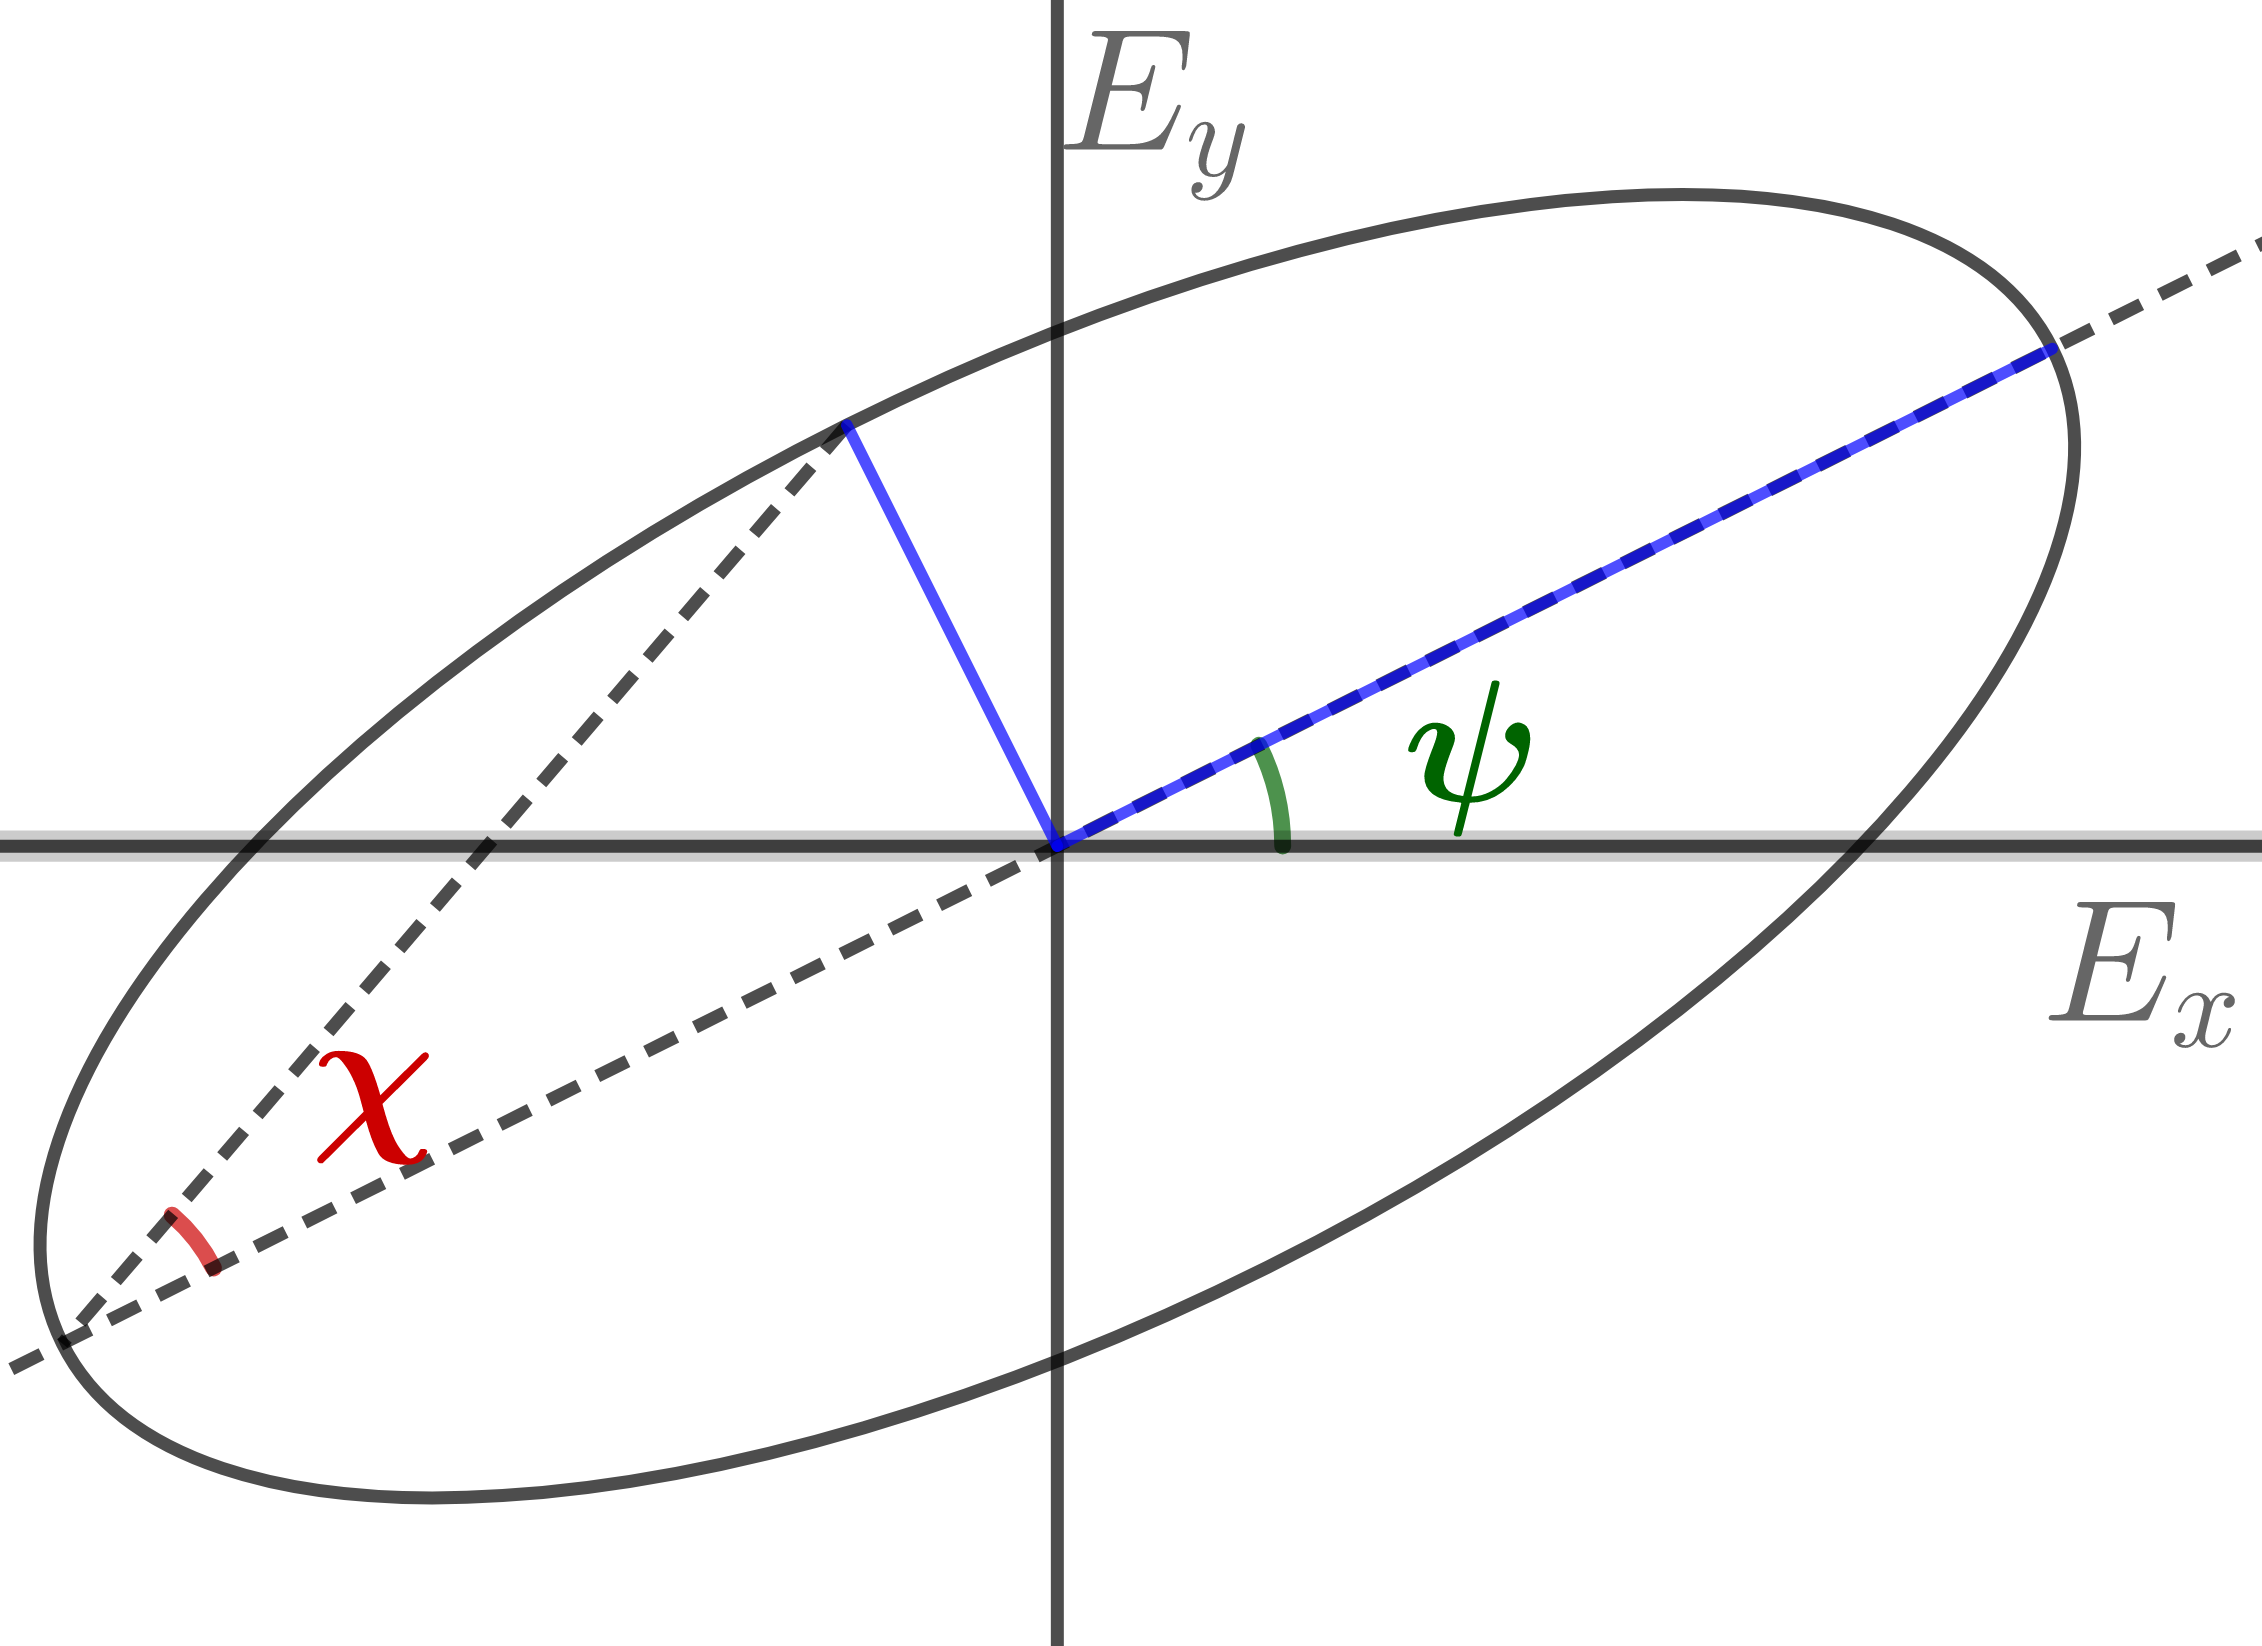
\includegraphics[width=0.96\textwidth]{ellipse beamer}
		\column{0.45\textwidth}
			\centering \textit{Poincare sphere}
			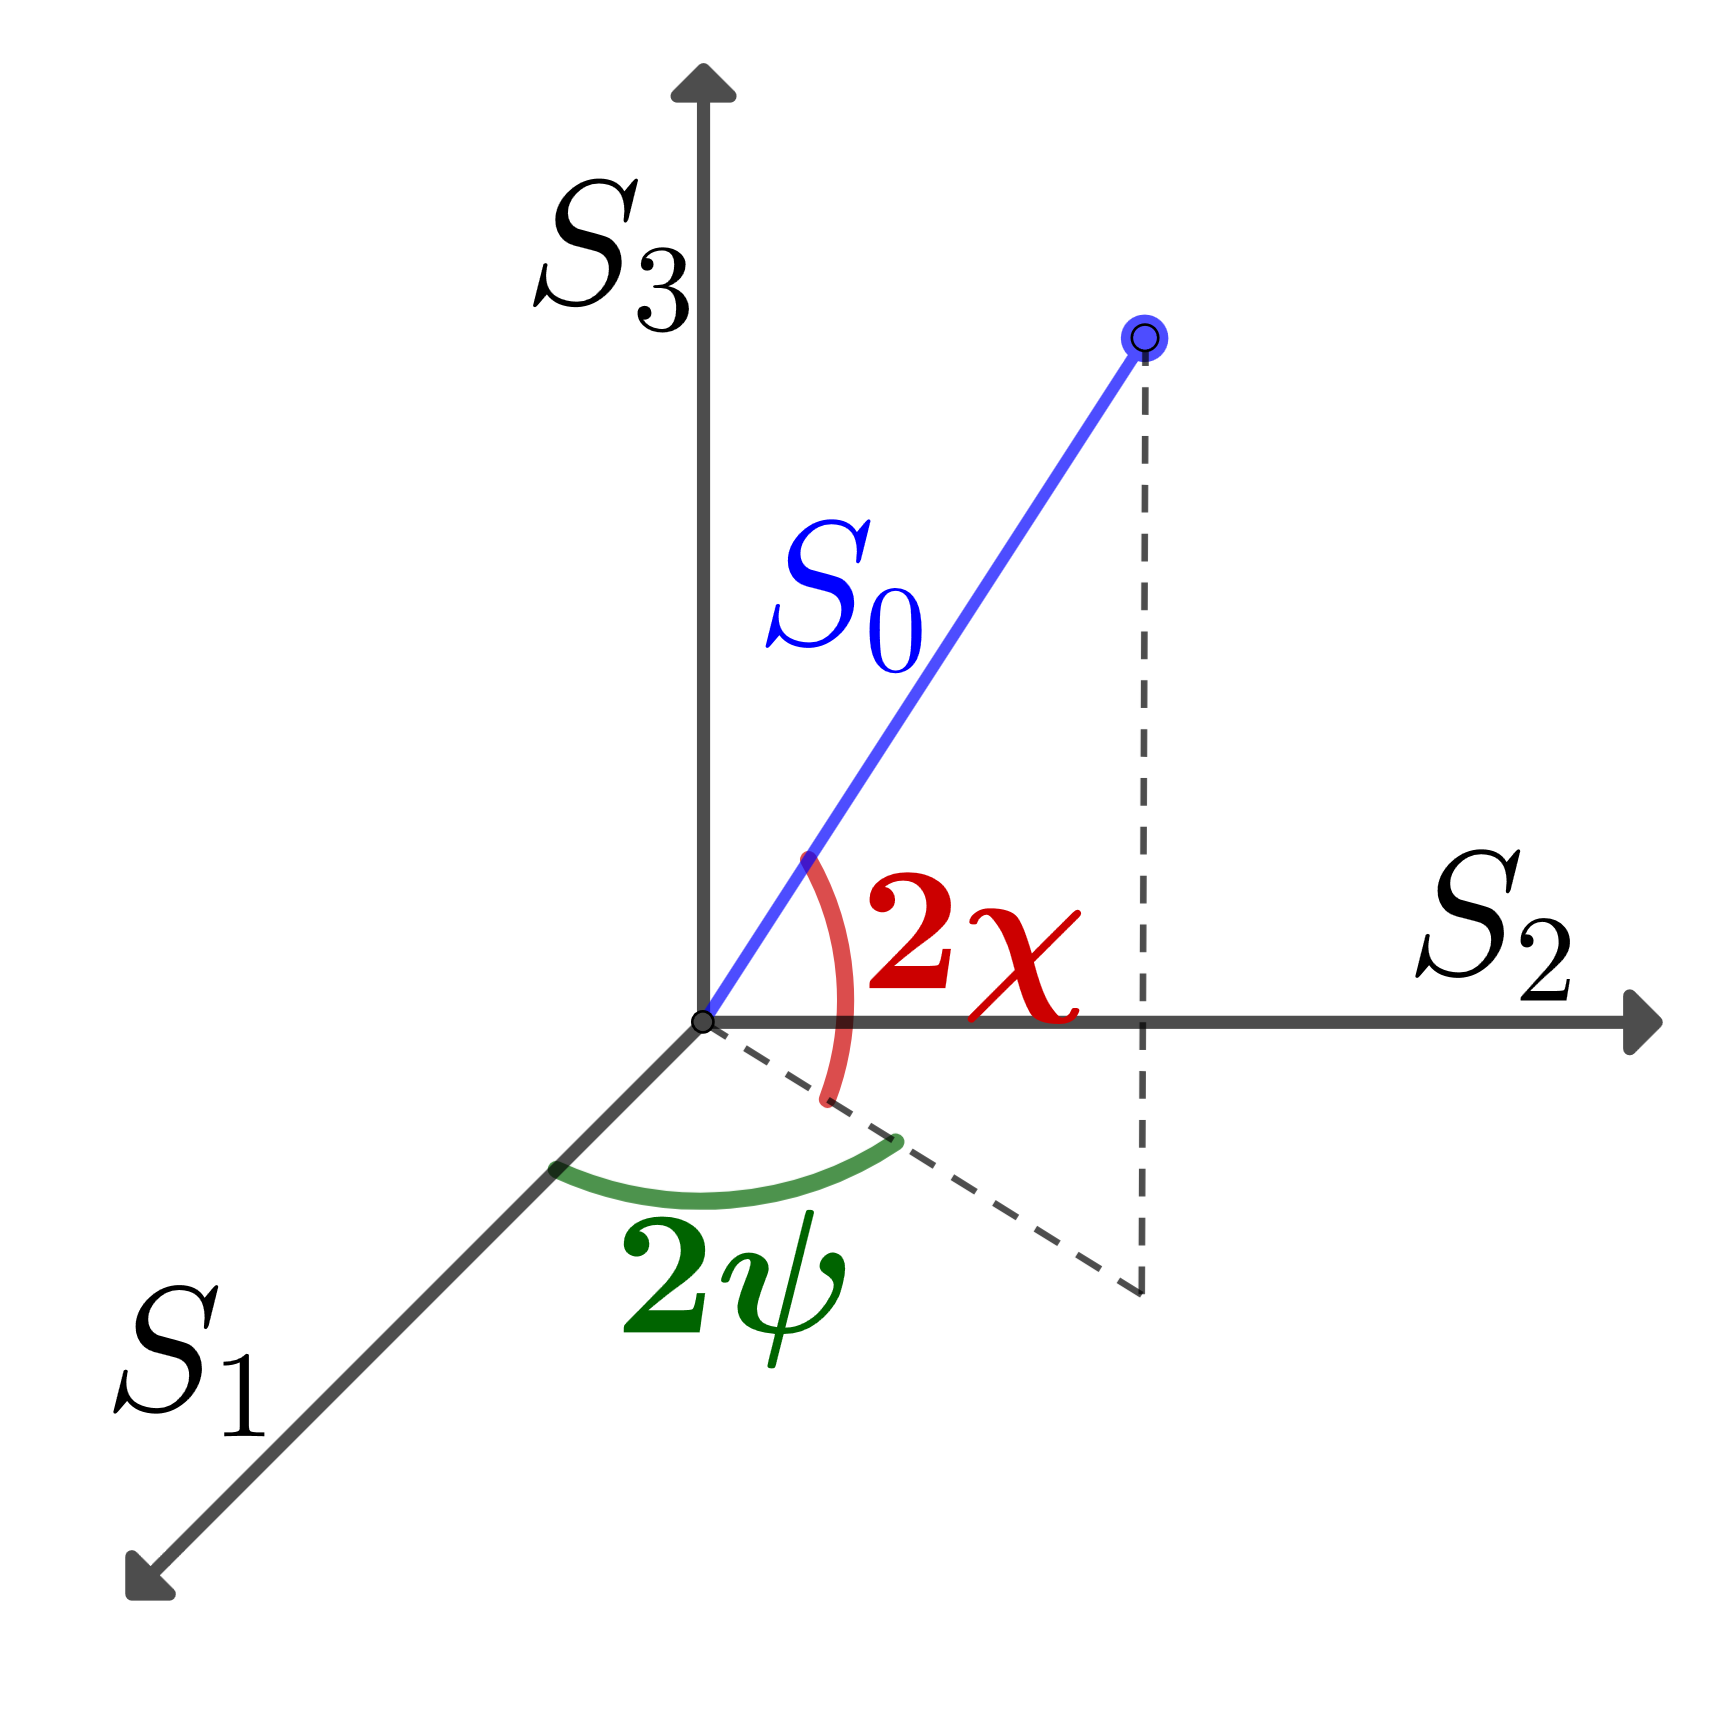
\includegraphics[width=0.72\textwidth]{poincare beamer}
	\end{columns}}

\end{frame}

\begin{frame}[t]{Poincare sphere representation}
For un-polarized light,
	\begin{align*}\boldsymbol{S}=
		S_0
		\begin{bmatrix}
			1\\
			0\\
			0\\
			0
		\end{bmatrix}\longrightarrow
		\underbrace{(0,0,0)}_{\text{At Origin}}
	\end{align*}\pause

For partially polarized light,
\begin{align*}\boldsymbol{S}=
	\begin{bmatrix}
		S_0\\
		S_1\\
		S_2\\
		S_3
	\end{bmatrix}\longrightarrow
	\underbrace{(S_1,S_2,S_3)}_{\begin{matrix}
			\text{Inside sphere \textit{s.t.}}\\
			0<S_1^2+S_2^2+S_3^2<S_0^2
		\end{matrix}}
\end{align*}

\end{frame}

\section{Gaussian Beam}

\begin{frame}
	\centering
	\alert{\huge Gaussian Beam and properties}
	\begin{itemize}\Large
		\item<1>Paraxial wave
		\item<0>Gaussian beam solution and properties
		\item<0>Modes of Gaussian beam
	\end{itemize}
\end{frame}

\begin{frame}{Paraxial wave}\vspace{-4pt}
	Maxwell's wave equation: 
	$$\nabla^2\boldsymbol{E}(\boldsymbol{r},t) - \frac{1}{c^2} \frac{\partial^2}{\partial t^2} \boldsymbol{E}(\boldsymbol{r},t)=0$$\pause
	Paraxial beam propagating predominantly in $z$-direction, $$\boldsymbol{E}(x,y,z,t)= \boldsymbol{\psi}(x,y,z) e^{i(\omega t-kz)}$$\pause
	and taking slowly varying amplitude approx. \textit{i.e.}  $$\left|\frac{\partial^2\boldsymbol{\psi}}{\partial z^2}\right|\ll k \left|\frac{\partial\boldsymbol{\psi}}{\partial z}\right| \ll
	k^2\left|\boldsymbol{\psi}\right|$$\pause
	\textbf{Paraxial wave equation}:
	$${\color{blue}\frac{\partial^2\boldsymbol{\psi}}{\partial x^2}+\frac{\partial^2\boldsymbol{\psi}}{\partial y^2} -2ik \frac{\partial\boldsymbol{\psi}}{\partial r}=0}$$\pause
	One of the solutions is \alert{\Large Gaussian beam}.\vspace{6pt}
\end{frame}

\begin{frame}
	\centering
	\alert{\huge Gaussian Beam}
	\begin{itemize}\Large
		\item<0>Paraxial wave
		\item<1>Gaussian beam solution and properties
		\item<0>Modes of Gaussian beam
	\end{itemize}
\end{frame}

\begin{frame}[t]{Gaussian beam solution }\vspace{-16pt}
	$$\text{Ansatz: }\psi(\boldsymbol{r},z)= A \exp\left[-i\left(p(z) + \frac{kr^2}{2q(z)}\right)\right]$$\pause
	$$\psi(\boldsymbol{r},z)=A
	\only{\left(\frac{w_0}{w(z)}\right)}
	\exp(
	{\tan[-1](\frac{z}{z_0})}\;
	{-\;i\frac{kr^2}{2R(z)}}\;
	{-\;\frac{r^2}{w^2(z)}}
	)$$\pause
	
	\only<3>{\vspace{10pt}{\begin{columns}
				\column{0.5\textwidth}\centering \textit{Electric field}
				\includegraphics[width=\linewidth]{"rad of cur beamer"}
				\column{0.5\textwidth}\centering \textit{Intensity}
				\includegraphics[width=\linewidth]{"intensity_var beamer"}
	\end{columns}}}
\end{frame}

\begin{frame}[t]{Gaussian beam properties}\vspace{-16pt} %1
	$$\psi(\boldsymbol{r},z)=A
	{\underbrace{\left(\frac{\alert{w_0}}{w(z)}\right)}_{\text{term I}}}
	\exp(
	{i\tan[-1](\frac{z}{z_0})}\;
	{-i\frac{kr^2}{2R(z)}}\;
	{-\frac{r^2}{w^2(z)}}
	)$$
{Term I related to \textbf{spreading of beam}.\\\vspace{5pt}\pause
	\begin{columns}
	\column{0.4\textwidth}
	$w\rightarrow$ Physical radius\\\pause
	{\color{red}$w_0\rightarrow$ Beam waist}\pause
	$$w(z)= w_0\sqrt{1+\left(\frac{z}{z_0}\right)^2}$$\pause
	$z_0\rightarrow$ Rayleigh length
	$$ z_0 = \frac{\pi w_0^2}{\lambda}$$ 
	
	
	\column{0.5\textwidth}\only<2->{\includegraphics[width=\linewidth]{"beam waist beamer"}}
\end{columns}}

\end{frame}

\begin{frame}[t]{Gaussian beam properties}\vspace{-16pt} %2
	$$\psi(\boldsymbol{r},z)=A
	{\left(\frac{w_0}{w(z)}\right)}
	\exp(
	{\underbrace{i{\:}{\color{blue}\tan[-1](\frac{z}{z_0})}}_{\text{term II}}}\;
	{-i\frac{kr^2}{2R(z)}}\;
	{-\frac{r^2}{w^2(z)}}
	)$$
	
	{Term II related to \textbf{Gouy phase} ($\phi_G$).\\\pause
		\begin{columns}
			\column{0.4\textwidth}
			{\color{blue}$$\phi_G = \tan[-1](\frac{z}{z_0})$$}\pause
			\column{0.5\textwidth}\visible<3->{\includegraphics[width=0.9\linewidth]{"gouy beamer"}}
	\end{columns}}
\end{frame}

\begin{frame}[t]{Gaussian beam properties}\vspace{-16pt} %3
	$$\psi(\boldsymbol{r},z)=A
	{\left(\frac{w_0}{w(z)}\right)}
	\exp(
	{i\tan[-1](\frac{z}{z_0})}\;
	{\underbrace{-i\frac{kr^2}{2{\color{blue}R(z)}}}_{\text{term III}}}\;
	{-\frac{r^2}{w^2(z)}}
	)$$
	
	{Term III related to \textbf{radius of curvature} ($R$) of beam wave-front.\\\pause
		\begin{columns}
			\column{0.4\textwidth}
			{\color{blue}$$R(z)= z\left[1+\left(\frac{z_0}{z}\right)^2\right]$$} \pause
			\column{0.5\textwidth}\visible<3>{\includegraphics[width=\linewidth]{"R_vs_z beamer"}}
	\end{columns}}
\end{frame}

\begin{frame}[t]{Gaussian beam properties}\vspace{-16pt} %4
	$$\psi(\boldsymbol{r},z)=A
	{\left(\frac{w_0}{w(z)}\right)}
	\exp(
	{i\tan[-1](\frac{z}{z_0})}\;
	{-i\frac{kr^2}{2R(z)}}\;
	{\underbrace{\color{red}-\frac{r^2}{w^2(z)}}_{\text{term IV}}}
	)$$
	
	{Term IV related to \textbf{Gaussian intensity profile}.\pause
		\begin{columns}
			\column{0.4\textwidth}
				$$\color{red}I(r,z)\sim \exp(-\frac{2r^2}{w^2(z)})$$\pause
			
			\column{0.5\textwidth}
			\visible<3>{\includegraphics[width=\linewidth]{"intensity beamer"}}
	\end{columns}}
\end{frame}







\begin{frame}[t]{$q$ parameter and beam tracing}
	$$\psi(\boldsymbol{r},z)= A \exp\left[-i\left(p(z) + \frac{kr^2}{2\:{\color{red}q(z)}}\right)\right]$$\pause
	$\color{red}q(z)$ $\longrightarrow$ characteristic of a beam if $\lambda$ known.\pause
	\begin{align*}
		q(z) &= z + i\:\color{blue}z_0\\
		\frac{1}{q(z)} &= \frac{1}{\color{blue}R(z)} - i\: \frac{\lambda}{\pi\: \color{blue}w^2(z)}
	\end{align*}\pause

\begin{align*}\onslide<4->{{\color{red}q_{in}}\longrightarrow
	\underbrace{\boxed{\color{violet}{\begin{bmatrix}
		A&B\\
		C&D
	\end{bmatrix}}}}_{\begin{matrix}\text{Optical}\\ \text{element} \end{matrix}}
	\longrightarrow {\color{red}q_{out}}} \onslide<5>{= \frac{{\color{violet}A} {\color{red}q_{in}}+{\color{violet}B}}{{\color{violet}C} {\color{red}q_{in}}+ {\color{violet}D}}}
\end{align*}
\end{frame}

\begin{frame}
	\centering
	\alert{\huge Gaussian Beam and properties}
	\begin{itemize}\Large
		\item<0>Paraxial wave
		\item<0>Gaussian beam solution and properties
		\item<1>Modes of Gaussian beam
	\end{itemize}
\end{frame}

\begin{frame}[c]{Hermite-Gaussian mode}
	\begin{align*}
		\psi_{m,n}(\boldsymbol{r},z)=& A \left(\frac{w_0}{w(z)}\right) H_m\left(\frac{\sqrt{2} x}{w(z)}\right) H_n\left(\frac{\sqrt{2} y}{w(z)}\right)\exp( -\frac{r^2}{w^2(z)}) \cdot\nonumber\\ 
		&\exp( i\:(m+n+1)\tan[-1](\frac{z}{z_0}) -i\frac{kr^2}{2R(z)})
	\end{align*}\pause
	$m,n=0\;\Rightarrow\;\psi=$ \alert{Gaussian}
\end{frame}

\begin{frame}[t]{Hermite-Gaussian Intensity profile}
	\begin{figure}
		\foreach \n in {0,1,2,3}{
			\foreach \m in {0,1,2}{
				\ifthenelse{\n<3}{
					\begin{subfigure}[htbp]{0.3\textwidth}
						\centering
						\includegraphics[width=0.8\textwidth]{intensity_hg\n\m}
						\caption{$TEM_{\n\m}$}
						%\label{fig:hg\n\m}
					\end{subfigure}
					\hfill
				}
			}
		}
	\end{figure}
\end{frame}

\begin{frame}[t]{Laguerre-Gaussian mode}
	\begin{align*}
		\psi_{p,l}(r,\phi,z)=&A\:\frac{w_0}{w(z)} 	\left[\frac{r\sqrt{2}}{w(z)}\right]^{|l|} L_p^{|l|}\left(\frac{2r^2}{w^2(z)}\right)\exp(-\frac{r^2}{w^2(z)}) \cdot\nonumber\\ &\exp(\only<1,2>{-il\phi}\only<3>{{\color{blue}-il\phi}}+i(2p+l+1)\tan[-1](\frac{z}{z_0})-i\frac{kr^2}{2R(z)}) 
	\end{align*}\pause
	\only<1,2>{$l,p=0\;\Rightarrow\;\psi=$ \alert{Gaussian}}\pause
	\begin{columns}
		\column{0.5\textwidth}
		$\color{blue}\exp(-il\phi)\longrightarrow$ Helical phase\\ \hspace{75pt}(carries OAM)
		
		\column{0.5\textwidth}\visible<3->{\centering \textit{Helical phase front}\\\vspace{3mm} 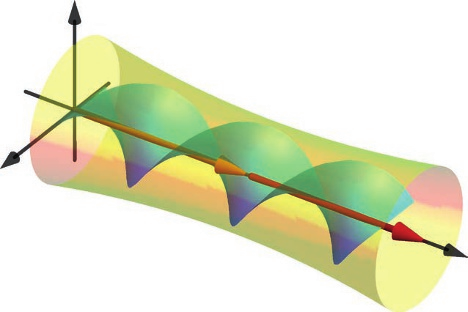
\includegraphics[width=0.7\textwidth]{ioam}}
	\end{columns}
\end{frame}

\begin{frame}[t]{Laguerre-Gaussian Intensity profile}
	\begin{figure}[t]
		\foreach \n in {0,1,2,3}{
			\foreach \m in {0,1,2}{
				\ifthenelse{\n<3}{
					\begin{subfigure}[htbp]{0.3\textwidth}
						\centering
						\includegraphics[width=0.8\textwidth]{intensity_lg\n\m}
						\caption{$p=\n,|l|=\m$}
						%\label{fig:hg\n\m}
					\end{subfigure}
					\hfill
				}
			}
		}
	\end{figure}
\end{frame}

\begin{frame}{Laguerre-Gaussian Phase profile}
	\begin{figure}
		\foreach \n in {0,1,2,3}{
			\foreach \m in {0,1,2}{
				\ifthenelse{\n<3}{
					\begin{subfigure}[htbp]{0.3\textwidth}
						\centering
						\includegraphics[width=0.8\textwidth]{phase_lg\n\m}
						\caption{$p=\n,l=\m$}
						%\label{fig:hg\n\m}
					\end{subfigure}
					\hfill
					}
				}
			}
		\end{figure}
\end{frame}



\end{document}